%%%%%%%%%%%%%%%%%%%%%%%%%%%%%%%%%%%%%%%%%
% University/School Laboratory Report
% LaTeX Template
% Version 3.1 (25/3/14)
%
% This template has been downloaded from:
% http://www.LaTeXTemplates.com
%
% Original author:
% Linux and Unix Users Group at Virginia Tech Wiki 
% (https://vtluug.org/wiki/Example_LaTeX_chem_lab_report)
%
% License:
% CC BY-NC-SA 3.0 (http://creativecommons.org/licenses/by-nc-sa/3.0/)
%
%%%%%%%%%%%%%%%%%%%%%%%%%%%%%%%%%%%%%%%%%

%----------------------------------------------------------------------------------------
%	PACKAGES AND DOCUMENT CONFIGURATIONS
%----------------------------------------------------------------------------------------

\documentclass{article}

\usepackage[version=3]{mhchem} % Package for chemical equation typesetting
\usepackage{siunitx} % Provides the \SI{}{} and \si{} command for typesetting SI units
\usepackage{graphicx} % Required for the inclusion of images
\usepackage{natbib} % Required to change bibliography style to APA
\usepackage{amsmath} % Required for some math elements 
\usepackage{enumerate} % Required for the enumerate function
\usepackage[americanvoltages,siunitx]{circuitikz} % Required for the drawing of circuit diagrams
\usepackage{caption}
\usepackage{graphicx}
\usepackage{subcaption}
\usepackage{xfrac}
\usepackage{float}
\usepackage{enumitem}

\setlength\parindent{0pt} % Removes all indentation from paragraphs

\renewcommand{\labelenumi}{\alph{enumi}.} % Make numbering in the enumerate environment by letter rather than number (e.g. section 6)

%\usepackage{times} % Uncomment to use the Times New Roman font

%----------------------------------------------------------------------------------------
%	DOCUMENT INFORMATION
%----------------------------------------------------------------------------------------

\title{Electrical Circuit Analysis \\ Practical 4 - Band Pass Filters \\ ENG223} % Title

\author{Shane \textsc{Reynolds}} % Author name

\date{\today} % Date for the report

\begin{document}

\maketitle % Insert the title, author and date

\begin{center}
\begin{tabular}{l r}
Date Performed: & September 8, 2015 \\ % Date the experiment was performed
Instructor: & Dr Kamal Debnath % Instructor/supervisor
\end{tabular}
\end{center}

% If you wish to include an abstract, uncomment the lines below
% \begin{abstract}
% Abstract text
% \end{abstract}

%----------------------------------------------------------------------------------------
%	SECTION 1
%----------------------------------------------------------------------------------------

\section{Objective}

To develop an understanding of band-pass filter operation through the derivation of a theoretical transfer function, theoretical cut-off frequencies and theoretical bandwidth. Theoretical estimates will be tested through the collection of experimental evidence.

\subsection{Background}
\label{definitions}

\begin{description}
\item[Upper and lower cut off frequencies for an RC band pass filter]
Figure 1 shows a simple bandpass filter with the output voltage taken over the capacitor. This set-up can be thought of a high pass RC filter in the first stage, with a low pass RC filter in the second stage. This type of filter allows a spectrum of frequencies through with both low and high frequencies outside of this range being attenuated.

%Circuit Diagram
\begin{figure}[H]
	\centering
	\ctikzset {bipoles/length=.8cm}
	\begin{circuitikz}[scale=0.6]
		
		\draw (0,0)
		to [sV, l=$V_{in}$] (0,4)
		to [C, l=$C_1$] (4,4)
		to [R, l=$R_1$] (4,0)
		to [short] (0,0)
		;
		
		\draw (4,4)
		to [R, l=$R_2$] (8,4)
		to [C, v^<=$C_2$] (8,0)
		to [short] (4,0)
		;
		
	\end{circuitikz}
	\captionof{figure}{RC Band pass filter with Sinusoidal Input Voltage}
	\label{fig:figure2}
\end{figure}

Both the high pass and low pass sections of the bandpass filter have a cut off frequency which was derived in practicals 2 and 3. This is given by:

\begin{align*}
	\omega_c = \frac{1}{RC}
\end{align*}

Hence the lower cut off frequency in radians per second is given by:

\begin{align*}
	\omega_{c1} &= \frac{1}{R_1 C_1}\\
	&= \frac{1}{330 \times 0.47e^{-6}}\\
	&= 6447.45 \si{\sfrac{\radian}{\second}}
\end{align*}

The cut off frequency in hertz is:

\begin{align*}
	f_{c1} &= \frac{6447.45}{2 \pi}\\
	&= 1026.14 \si{\hertz} 
\end{align*}

The upper cut off frequency in radians per second is given by:

\begin{align*}
\omega_{c2} &= \frac{1}{R_2 C_2}\\
&= \frac{1}{330 \times 0.047e^{-6}}\\
&= 64474.53 \si{\sfrac{\radian}{\second}}
\end{align*}

The cut off frequency in hertz is:

\begin{align*}
f_{c2} &= \frac{64474.53}{2 \pi}\\
&= 10261.44 \si{\hertz} 
\end{align*}

The bandwidth, $\beta$, is calculated as follows:

\begin{align*}
	\beta &= \omega_{c2} - \omega_{c1} \\
	&= 64474.53 - 6447.45\\
	&= 58027.08 \si{\sfrac{\radian}{\second}}
\end{align*}

The transfer function for the filter can be found by considering the second stage of the filter first, and then the first stage. Consider the impedence of the resistors as $Z_R = R$, the resistance of the first stage capacitor as $Z_{C1} = \sfrac{1}{j \omega C1}$ and the second stage capacitor as $Z_{C2} = \sfrac{1}{j \omega C2}$. The output voltage can be found as a function of the voltage across $R_1$, using the voltage divider, that is:

\begin{align*}
	V_o &= \frac{Z_{C2}}{Z_R + Z_{C2}} \times V_{R1}
\end{align*}

Now, the voltage across the resistor $R_1$ is given by:

\begin{align*}
	V_{R1} = \frac{Z_{R}}{Z_{R} + Z_{C1}} \times V_i
\end{align*}

Hence, substituting the expression for $V_R$ into the expression for $V_o$, we get the following:

\begin{align*}
	V_o &= \frac{Z_{C2}}{Z_R + Z_{C2}} \times \frac{Z_{R}}{Z_{R} + Z_{C1}} \times V_i
\end{align*}

Hence, our transfer function is given by:

\begin{align}
	\frac{V_o}{V_i} &= \frac{Z_{C2}}{Z_R + Z_{C2}} \times \frac{Z_{R}}{Z_{R} + Z_{C1}} \nonumber \\
	&= \frac{\frac{1}{j \omega C_2}}{R + \frac{1}{j \omega C_2}} \times \frac{R}{R + \frac{1}{j \omega C_1}} \nonumber\\
	&= \frac{1}{1 + j \omega C_2 R} \times \frac{R}{R - j \frac{1}{\omega C_1}}
\end{align}

In phasor form the transfer function is:

\begin{align*}
	H(\omega) &= \bigg(\frac{1}{\sqrt{1 + (\omega C_2 R)^2}}\bigg) \bigg(\frac{R}{\sqrt{R^2 + (\frac{1}{\omega C_1})^2}}\bigg) \angle (-\arctan(\omega C_2 R) - \arctan(\frac{-1}{\omega R C_1}))
\end{align*}

The magnitude of the transfer function is given by:

\begin{align}
	|H(\omega)| &= \bigg(\frac{1}{\sqrt{1 + (\omega C_2 R)^2}}\bigg) \bigg(\frac{R}{\sqrt{R^2 + (\sfrac{1}{\omega C_1})^2}}\bigg)
\end{align}

The phase of the transfer function is given by:

\begin{align}
	\theta(\omega) = (-\arctan(\omega C_2 R) - \arctan(\sfrac{-1}{\omega R C_1}))
\end{align}

A plot of both the magnitude of the transfer function, equation (2), and the phase angle, equation (3), can be seen in figure 2.

\begin{center}
	\begin{figure}[H]
		\begin{minipage}{0.6\textwidth}
			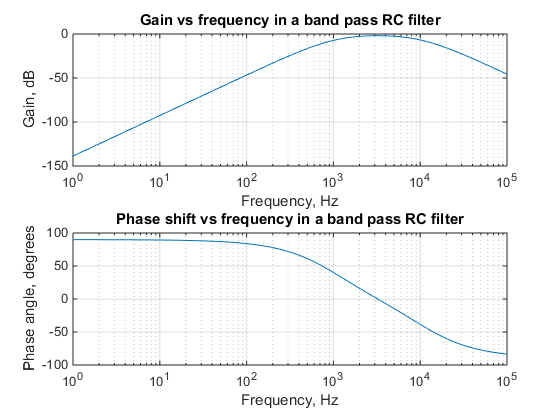
\includegraphics[scale=0.8]{bode1}
			\captionof{figure}{Theoretical bode plots for band pass RC filter}
		\end{minipage}
	\end{figure}
\end{center}

\end{description} 

\newpage

%----------------------------------------------------------------------------------------
%	SECTION 2
%----------------------------------------------------------------------------------------

\section{Experimental Circuit Set-up, Results and Calculations}

The RC band pass filter circuit was set up as shown in figure 3. The input voltage, $V_{in}$, was a sinusoidal voltage source generated by the function generator. The output voltage, $V_{out}$, was measured across the second capacitor.

%Circuit Diagram
\begin{figure}[H]
	\centering
	\ctikzset {bipoles/length=.8cm}
	\begin{circuitikz}[scale=0.6]
		
		\draw (0,0)
		to [sV, l=$V_{in}$] (0,4)
		to [C, l=0.47\si{\micro\farad}] (4,4)
		to [R, l=330\si{\ohm}] (4,0)
		to [short] (0,0)
		;
		
		\draw (4,4)
		to [R, l=330\si{\ohm}] (8,4)
		to [C, v^<=0.047\si{\micro\farad}] (8,0)
		to [short] (4,0)
		;
		
	\end{circuitikz}
	\captionof{figure}{RC Band pass filter with Sinusoidal Input Voltage}
	\label{fig:figure2}
\end{figure}

The input voltage, $V_{in}$, was set to 4V peak to peak. Both the output voltage, $V_{out}$, and the time difference between the input signal peak and output signal peak, $|\Delta X|$, were measured. The gain and phase shift were calculated using the formulas from practical 1. The empirical data and calculated values can be seen in table 1.
 
\begin{figure}[H]
\centering
\begin{tabular}{ | r | r | r | r | r | r | }
	\hline
	frequency ($f$) & $V_{in}$ & $V_{out}$ & $|\Delta X|$ & Gain $\si{\decibel}$ & Phase Shift $\si{\degree}$ \\ \hline
	100 \si{\hertz} & 4 \si{\volt} & 408 \si{\milli\volt} & 2.24\si{\milli\second} (out lead in) & -19.288 \si{\decibel} & 80.64 \si{\degree}\\ \hline
	200 \si{\hertz} & 4 \si{\volt} & 784 \si{\milli\volt} & 1.12 \si{\milli\second} (out lead in) & -14.155 \si{\decibel} & 80.64 \si{\degree}\\ \hline
	500 \si{\hertz} & 4 \si{\volt} & 1.74 \si{\volt} & 328 \si{\micro\second} (out lead in) & -7.230 \si{\decibel} & 59.04 \si{\degree}\\ \hline
	1000 \si{\hertz} & 4 \si{\volt} & 2.68 \si{\volt} & 108 \si{\micro\second} (out lead in) & -3.479 \si{\decibel} & 38.88 \si{\degree}\\ \hline
	2000 \si{\hertz} & 4 \si{\volt} & 3.24 \si{\volt} & 22 \si{\micro\second} (out lead in) & -1.830 \si{\decibel} & 15.84 \si{\degree}\\ \hline
	4000 \si{\hertz} & 4 \si{\volt} & 3.28 \si{\volt} & 6.40 \si{\micro\second} (in lead out) & -1.724 \si{\decibel} & -9.22 \si{\degree}\\ \hline
	5000 \si{\hertz} & 4 \si{\volt} & 3.22 \si{\volt} & 8.00 \si{\micro\second} (in lead out) & -1.884 \si{\decibel} & -14.40 \si{\degree}\\ \hline
	8000 \si{\hertz} & 4 \si{\volt} & 2.96 \si{\volt} & 12 \si{\micro\second} (in lead out) & -2.615 \si{\decibel} & -34.56 \si{\degree}\\ \hline
	10000 \si{\hertz} & 4 \si{\volt} & 2.76 \si{\volt} & 11.6 \si{\micro\second} (in lead out) & -3.223 \si{\decibel} & -41.76 \si{\degree}\\ \hline
	20000 \si{\hertz} & 4 \si{\volt} & 1.88 \si{\volt} & 8.40 \si{\micro\second} (in lead out) & -6.558 \si{\decibel} & -60.48 \si{\degree}\\ \hline
	50000 \si{\hertz} & 4 \si{\volt} & 860 \si{\milli\volt} & 4.32 \si{\micro\second} (in lead out) & -13.351 \si{\decibel} & -77.76 \si{\degree}\\ \hline
	100000 \si{\hertz} & 4 \si{\volt} & 432 \si{\milli\volt} & 2.44 \si{\micro\second} (in lead out) & -19.332 \si{\decibel} & -87.84 \si{\degree}\\ \hline
\end{tabular}
\captionof{table}{Output characteristics for an RC band pass filter circuit}
\end{figure}

The maximum voltage gain in achieved from the circuit was found by scanning near the highest frequency in the table. The frequency at which the highest voltage was found was:

\begin{align*}
	f_c = 3250\si{\hertz}
\end{align*} 

The maximum voltage with an input at $f_c$ is:

\begin{align*}
	V_{f0} = 3.34\si{\volt}
\end{align*}

By adjusting the frequency of the function generator until the output voltage had an amplitude of 70.7\% of its maximum value, the lower cut off frequency was measured. The measured value was:

\begin{align*}
	f_1 = 750 \si{\hertz}
\end{align*}

The voltage at the lower cut off point was:

\begin{align*}
	V_{f1} = 2.32\si{\volt}
\end{align*}

The same was done to measure the upper cut off frequency. The measured value was:

\begin{align*}
	f_2 = 12850\si{\hertz}
\end{align*}

The voltage at this frequency was:

\begin{align*}
	V_{f2} = 2.32\si{\volt}
\end{align*}

\newpage

%----------------------------------------------------------------------------------------
%	SECTION 3
%----------------------------------------------------------------------------------------

\section{Results and Conclusions}

The gain and phase angle calculations made for the empirical data shown in table 1 for the RC band pass filter circuit was plotted over the theoretical plots. This can be seen in figure 4.

\begin{center}
	\begin{figure}[H]
		\begin{minipage}{0.6\textwidth}
			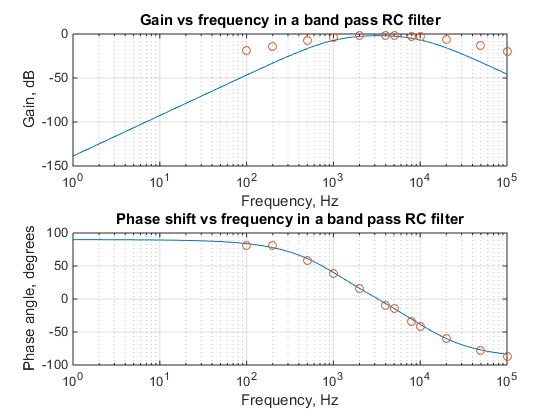
\includegraphics[scale=0.8]{bode2}
			\captionof{figure}{Empirical data super-imposed on theoretical data for low pass RC filter}
		\end{minipage}
	\end{figure}
\end{center}

The observed phase shift matches closely to the theoretical expectation, however, the magnitude plots shows some divergence from theoretical values. The theoretical centre frequency can be determined using the geometric mean of the upper and lower theoretical cut off frequencies:

\begin{align*}
	\omega_c &= \sqrt{\omega_{c1} \times \omega_{c2}} \\
	&= \sqrt{1026.14 \times 10261.44} \\
	&= 3244.94 \si{\hertz}
\end{align*}

This is roughly the same as the empirical centre frequency. There was, however, a material difference observed between the theoretical lower cut off frequency and the empirical value. Similarly, this was the case for the theoretical upper cut off and the measured value. As previously mentions, this divergence between theoretical and measured results can be seen in figure 4. Noticeably, as the frequencies get to the lower and upper positions of the spectrum, the divergence becomes more pronounced. One explanation for the divergence is that the wires that connect the circuit elements are not ideal, that is, they carry some resistance. Further, there may be parasitic capacitive or inductive effects that are causing the results to deviate from the theoretical expectations.

%----------------------------------------------------------------------------------------
%	BIBLIOGRAPHY
%----------------------------------------------------------------------------------------


%----------------------------------------------------------------------------------------


\end{document}